%==============================================================================
% PART 5: RDT2-FM ARCHITECTURE
%==============================================================================

\section{RDT2-FM Architecture}

%------------------------------------------------------------------------------
\begin{frame}{RDT2-FM Overview}
    \begin{block}{Definition}
        \textbf{RDT2-FM} = Frozen VLM + Flow-Matching Action Expert
    \end{block}

    \vspace{0.5cm}
    \textbf{Core Architecture:}
    \begin{itemize}
        \item \textbf{VLM Backbone:} Qwen2.5-VL-7B-Instruct (\textbf{frozen})
        \item \textbf{Action Expert:} 400M parameter RDT transformer
        \item \textbf{Generation:} Flow-matching diffusion (5 steps)
    \end{itemize}

    \vspace{0.5cm}
    \begin{alertblock}{Key Advantage}
        \textbf{6 forward passes} total (1 VLM + 5 RDT) \\
        $\sim$4.5$\times$ faster than RDT2-VQ
    \end{alertblock}
\end{frame}

%------------------------------------------------------------------------------
\begin{frame}{Architecture Comparison}
    \begin{table}
        \centering
        \renewcommand{\arraystretch}{1.4}
        \begin{tabular}{lcc}
            \toprule
            & \textbf{RDT2-VQ} & \textbf{RDT2-FM} \\
            \midrule
            VLM Backbone & Fine-tuned & \textbf{Frozen} \\
            Action Output & Discrete (27 tokens) & \textbf{Continuous} \\
            Forward Passes & 27 & \textbf{6} \\
            Trainable Params & 7B+ & \textbf{400M} \\
            Training VRAM & $\geq$32 GB & \textbf{$\sim$16 GB} \\
            \bottomrule
        \end{tabular}
    \end{table}

    \vspace{0.5cm}
    \begin{block}{Key Insight}
        Freeze VLM $\rightarrow$ Only train lightweight action expert \\
        Same visual understanding, much faster training
    \end{block}
\end{frame}

%------------------------------------------------------------------------------
\begin{frame}{RDT2-FM Architecture Diagram}
    \begin{center}
    \begin{tikzpicture}[
        box/.style={rectangle, draw, rounded corners, minimum width=2cm, minimum height=0.7cm, align=center, font=\scriptsize},
        arrow/.style={->, thick},
        scale=0.75, transform shape
    ]
        % Input
        \node[box, fill=blue!20] (img) at (0,4) {Images\\$384 \times 768$};
        \node[box, fill=green!20] (inst) at (3,4) {Instruction};

        % Frozen VLM
        \node[box, fill=qwenblue!30, minimum width=5cm] (qwen) at (1.5,2) {Qwen2.5-VL (Frozen)};
        \node[box, fill=yellow!30] (kv) at (1.5,0) {KV Cache\\Hidden States};

        % RDT Expert
        \node[box, fill=rdtgreen!30, minimum width=4cm] (rdt) at (8,2) {RDT Action Expert\\(400M params)};

        % State input
        \node[box, fill=actionorange!30] (state) at (8,4) {Robot State\\$[1, 20]$};

        % Noise
        \node[box, fill=gray!30] (noise) at (12,4) {Noise\\$\mathcal{N}(0, I)$};

        % Output
        \node[box, fill=vqpurple!30] (action) at (8,0) {Action\\$[24, 20]$};

        % Arrows
        \draw[arrow] (img) -- (qwen);
        \draw[arrow] (inst) -- (qwen);
        \draw[arrow] (qwen) -- (kv);
        \draw[arrow] (kv) -- node[above] {condition} (rdt);
        \draw[arrow] (state) -- (rdt);
        \draw[arrow] (noise) -- (rdt);
        \draw[arrow] (rdt) -- node[right] {5 steps} (action);

        % Frozen indicator
        \node[draw, dashed, blue, fit=(qwen), inner sep=3pt] {};
        \node[blue, font=\tiny] at (1.5,2.8) {Frozen};
    \end{tikzpicture}
    \end{center}
\end{frame}

%------------------------------------------------------------------------------
\begin{frame}{Flow Matching: Overview}
    \begin{block}{Core Idea}
        Learn to transport samples from noise distribution to data distribution
    \end{block}

    \vspace{0.3cm}
    \textbf{Probability Flow ODE:}
    \[
        \frac{d\vect{x}_t}{dt} = \vect{v}_\theta(\vect{x}_t, t)
    \]

    where $\vect{v}_\theta$ is the learned velocity field

    \vspace{0.5cm}
    \textbf{Interpolation Path (Linear):}
    \[
        \vect{x}_t = (1 - t) \cdot \vect{x}_0 + t \cdot \vect{x}_1
    \]

    \begin{itemize}
        \item $t = 0$: Pure noise $\vect{x}_0 \sim \mathcal{N}(0, I)$
        \item $t = 1$: Data sample $\vect{x}_1 = \vect{a}_{\text{gt}}$
    \end{itemize}

    \vspace{0.3cm}
    \textbf{Target Velocity:}
    \[
        \vect{v}^* = \vect{x}_1 - \vect{x}_0 = \vect{a}_{\text{gt}} - \boldsymbol{\epsilon}
    \]
\end{frame}

%------------------------------------------------------------------------------
\begin{frame}{Flow Matching: Training Loss}
    \textbf{Objective: Learn to predict velocity}

    \vspace{0.5cm}
    \textbf{Training Procedure:}
    \begin{enumerate}
        \item Sample noise: $\boldsymbol{\epsilon} \sim \mathcal{N}(0, I)$
        \item Sample timestep: $t \sim \text{LogisticNormal}(\mu, \sigma)$
        \item Create noisy action: $\vect{a}_t = (1 - t) \cdot \boldsymbol{\epsilon} + t \cdot \vect{a}_{\text{gt}}$
        \item Predict velocity: $\hat{\vect{v}} = f_\theta(\vect{a}_t, t, \text{cond})$
        \item Compute loss: $\mathcal{L} = \|\hat{\vect{v}} - (\vect{a}_{\text{gt}} - \boldsymbol{\epsilon})\|^2$
    \end{enumerate}

    \vspace{0.5cm}
    \textbf{Flow Matching Loss:}
    \[
        \boxed{\mathcal{L}_{\text{FM}} = \mathbb{E}_{t, \boldsymbol{\epsilon}, \vect{a}} \left[ \| \vect{v}_\theta(\vect{a}_t, t) - (\vect{a} - \boldsymbol{\epsilon}) \|^2 \right]}
    \]
\end{frame}

%------------------------------------------------------------------------------
\begin{frame}{Timestep Sampling: Logistic Normal}
    \begin{block}{Why Not Uniform?}
        Different timesteps have different importance for learning
    \end{block}

    \vspace{0.3cm}
    \textbf{Logistic Normal Distribution:}
    \[
        t = \sigma\left(\frac{u - \mu}{\sigma}\right), \quad u \sim \mathcal{N}(0, 1)
    \]

    where $\sigma(x) = \frac{1}{1 + e^{-x}}$ (sigmoid)

    \vspace{0.3cm}
    \textbf{Default Parameters:}
    \begin{itemize}
        \item $\mu = 0$ (center)
        \item $\sigma = 1$ (spread)
    \end{itemize}

    \vspace{0.3cm}
    \begin{alertblock}{Effect}
        More samples near $t = 0.5$ (intermediate states) \\
        Fewer samples at extremes ($t \approx 0$ or $t \approx 1$)
    \end{alertblock}
\end{frame}

%------------------------------------------------------------------------------
\begin{frame}{Inference: Euler Integration}
    \textbf{Generate actions by integrating velocity field}

    \vspace{0.3cm}
    \textbf{Algorithm (5 steps):}
    \begin{algorithmic}[1]
        \State $\vect{a}_0 \sim \mathcal{N}(0, I)$ \Comment{Sample noise}
        \State $\Delta t \leftarrow 1 / N$ \Comment{$N = 5$ steps}
        \For{$i = 0$ to $N-1$}
            \State $t \leftarrow i \cdot \Delta t$
            \State $\vect{v} \leftarrow \vect{v}_\theta(\vect{a}_t, t, \text{cond})$ \Comment{RDT forward}
            \State $\vect{a}_{t + \Delta t} \leftarrow \vect{a}_t + \vect{v} \cdot \Delta t$ \Comment{Euler step}
        \EndFor
        \State \textbf{Return} $\vect{a}_1$
    \end{algorithmic}

    \vspace{0.5cm}
    \textbf{Timesteps:} $t \in \{0, 0.2, 0.4, 0.6, 0.8\} \rightarrow 1.0$
\end{frame}

%------------------------------------------------------------------------------
\begin{frame}{RDT Transformer Architecture}
    \begin{block}{RDT = Robotics Diffusion Transformer}
        Specialized transformer for action diffusion
    \end{block}

    \vspace{0.3cm}
    \textbf{Architecture Specifications:}
    \begin{table}
        \centering
        \renewcommand{\arraystretch}{1.2}
        \begin{tabular}{ll}
            \toprule
            \textbf{Parameter} & \textbf{Value} \\
            \midrule
            Hidden size & 1024 \\
            Depth (layers) & 14 \\
            Attention heads & 8 \\
            KV heads (GQA) & 4 \\
            Register tokens & 4 \\
            FFN multiplier & 256 \\
            Total params & $\sim$400M \\
            \bottomrule
        \end{tabular}
    \end{table}
\end{frame}

%------------------------------------------------------------------------------
\begin{frame}{RDT Block Structure}
    \begin{center}
    \begin{tikzpicture}[
        box/.style={rectangle, draw, rounded corners, minimum width=3cm, minimum height=0.6cm, align=center, font=\scriptsize},
        arrow/.style={->, thick},
        scale=0.85, transform shape
    ]
        % Input
        \node[box, fill=blue!20] (input) at (0,5) {Action Tokens\\$[B, 24, 1024]$};

        % Self-attention
        \node[box, fill=vqpurple!30] (sa) at (0,3.5) {Self-Attention};
        \node[box, fill=gray!30] (mod1) at (3.5,3.5) {adaLN\\(timestep)};

        % Cross-attention
        \node[box, fill=qwenblue!30] (ca) at (0,2) {Cross-Attention\\to VLM features};
        \node[box, fill=yellow!30] (cond) at (3.5,2) {KV Cache\\from Qwen};

        % FFN
        \node[box, fill=rdtgreen!30] (ffn) at (0,0.5) {SwiGLU FFN};
        \node[box, fill=gray!30] (mod2) at (3.5,0.5) {adaLN\\(timestep)};

        % Output
        \node[box, fill=blue!20] (output) at (0,-1) {Output\\$[B, 24, 1024]$};

        % Arrows
        \draw[arrow] (input) -- (sa);
        \draw[arrow] (mod1) -- (sa);
        \draw[arrow] (sa) -- (ca);
        \draw[arrow] (cond) -- (ca);
        \draw[arrow] (ca) -- (ffn);
        \draw[arrow] (mod2) -- (ffn);
        \draw[arrow] (ffn) -- (output);

        % Residual connections
        \draw[arrow, dashed] (input.west) -- ++(-0.5,0) |- (sa.west);
        \draw[arrow, dashed] (sa.west) -- ++(-0.3,0) |- (ca.west);
        \draw[arrow, dashed] (ca.west) -- ++(-0.3,0) |- (ffn.west);
    \end{tikzpicture}
    \end{center}

    \vspace{0.3cm}
    \textbf{adaLN:} Adaptive Layer Norm modulated by timestep embedding
\end{frame}

%------------------------------------------------------------------------------
\begin{frame}{Timestep Embedding}
    \textbf{Sinusoidal Frequency Encoding:}

    \vspace{0.3cm}
    \[
        \text{PE}(t, 2k) = \sin\left(\frac{t}{10000^{2k/d}}\right)
    \]
    \[
        \text{PE}(t, 2k+1) = \cos\left(\frac{t}{10000^{2k/d}}\right)
    \]

    \vspace{0.3cm}
    \textbf{MLP Processing:}
    \begin{lstlisting}[language=Python, basicstyle=\ttfamily\small]
class TimestepEmbedder(nn.Module):
    def __init__(self, hidden_size, freq_dim=256):
        self.mlp = nn.Sequential(
            nn.Linear(freq_dim, hidden_size),
            nn.SiLU(),
            nn.Linear(hidden_size, hidden_size)
        )
    \end{lstlisting}

    \vspace{0.3cm}
    \textbf{Dimension Flow:}
    \[
        t \in [0, 1] \xrightarrow{\text{sinusoidal}} [256] \xrightarrow{\text{MLP}} [1024]
    \]
\end{frame}

%------------------------------------------------------------------------------
\begin{frame}{Condition Adaptors}
    \textbf{Project VLM features to RDT hidden space}

    \vspace{0.5cm}
    \begin{center}
    \begin{tikzpicture}[
        box/.style={rectangle, draw, rounded corners, minimum width=2.5cm, minimum height=0.6cm, align=center, font=\scriptsize},
        arrow/.style={->, thick}
    ]
        \node[box, fill=qwenblue!30] (vlm) at (0,0) {VLM Hidden\\$[B, L, 2176]$};
        \node[box, fill=gray!30] (adapt) at (4,0) {img\_adaptor\\MLP3x\_SiLU};
        \node[box, fill=rdtgreen!30] (rdt) at (8,0) {RDT Input\\$[B, L, 1024]$};

        \draw[arrow] (vlm) -- (adapt);
        \draw[arrow] (adapt) -- (rdt);
    \end{tikzpicture}
    \end{center}

    \vspace{0.5cm}
    \textbf{Adaptor Types:}
    \begin{itemize}
        \item \code{mlp2x\_gelu}: $d \rightarrow 2d \rightarrow d$ with GELU
        \item \code{mlp3x\_silu}: $d \rightarrow 3d \rightarrow d$ with SiLU
    \end{itemize}

    \vspace{0.3cm}
    \textbf{Adaptors in RDT:}
    \begin{itemize}
        \item \code{img\_adaptor}: VLM features $\rightarrow$ RDT (2176 $\rightarrow$ 1024)
        \item \code{act\_adaptor}: Action $\rightarrow$ RDT (20 $\rightarrow$ 1024)
        \item \code{state\_adaptor}: State $\rightarrow$ RDT (20 $\rightarrow$ 1024)
    \end{itemize}
\end{frame}

%------------------------------------------------------------------------------
\begin{frame}{KV Cache Extraction}
    \textbf{Extract VLM hidden states for RDT conditioning}

    \vspace{0.3cm}
    \begin{lstlisting}[language=Python, basicstyle=\ttfamily\small]
# Forward through frozen VLM
with torch.no_grad():
    outputs = vision_language_model(
        **inputs,
        output_hidden_states=True
    )

# Extract selected layer outputs
selected_layers = list(range(14))  # All layers
hidden_states = [
    outputs.hidden_states[i]
    for i in selected_layers
]

# Stack and create KV cache
kv_cache = torch.stack(hidden_states, dim=1)
# Shape: [B, num_layers, seq_len, hidden_dim]
    \end{lstlisting}

    \vspace{0.3cm}
    \textbf{VLM Hidden Dim:} 2176 (Qwen2.5-VL specific)
\end{frame}

%------------------------------------------------------------------------------
\begin{frame}{Attention Mask}
    \textbf{Control which VLM tokens RDT attends to}

    \vspace{0.5cm}
    \textbf{Mask Structure:}
    \begin{center}
    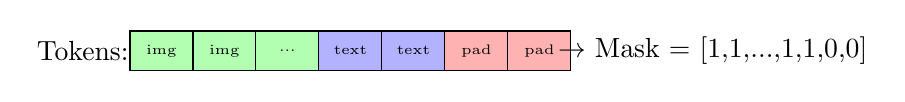
\begin{tikzpicture}[
        cell/.style={rectangle, draw, minimum width=0.8cm, minimum height=0.5cm, align=center, font=\tiny}
    ]
        \node[cell, fill=green!30] at (0,0) {img};
        \node[cell, fill=green!30] at (0.8,0) {img};
        \node[cell, fill=green!30] at (1.6,0) {...};
        \node[cell, fill=blue!30] at (2.4,0) {text};
        \node[cell, fill=blue!30] at (3.2,0) {text};
        \node[cell, fill=red!30] at (4.0,0) {pad};
        \node[cell, fill=red!30] at (4.8,0) {pad};

        \node at (-1,0) {Tokens:};
        \node at (7,0) {$\rightarrow$ Mask = [1,1,...,1,1,0,0]};
    \end{tikzpicture}
    \end{center}

    \vspace{0.5cm}
    \textbf{Implementation:}
    \begin{lstlisting}[language=Python, basicstyle=\ttfamily\small]
# Attention mask from processor
attn_mask = inputs["attention_mask"]  # [B, seq_len]

# Expand for cross-attention
# RDT action tokens attend to all valid VLM tokens
    \end{lstlisting}
\end{frame}

%------------------------------------------------------------------------------
\begin{frame}{RDT Forward Pass}
    \textbf{Single denoising step:}

    \vspace{0.3cm}
    \begin{lstlisting}[language=Python, basicstyle=\ttfamily\small]
def forward(self, gt_action, states, img_cond,
            img_attn_mask, lang_cond=None):
    # 1. Sample timesteps
    t = self.sample_timesteps(batch_size)

    # 2. Create noisy actions
    noise = torch.randn_like(gt_action)
    noisy_action = (1 - t) * noise + t * gt_action

    # 3. Predict velocity
    pred_velocity = self.model(
        x=noisy_action,
        t=t,
        img_cond=img_cond,
        img_mask=img_attn_mask,
        states=states
    )

    # 4. Compute loss
    target = gt_action - noise
    loss = F.mse_loss(pred_velocity, target)
    return loss
    \end{lstlisting}
\end{frame}

%------------------------------------------------------------------------------
\begin{frame}{RDT Inference}
    \textbf{Generate action from noise:}

    \vspace{0.3cm}
    \begin{lstlisting}[language=Python, basicstyle=\ttfamily\small]
def predict_action(self, states, img_cond,
                   img_attn_mask):
    B = states.shape[0]

    # Initialize with noise
    action = torch.randn(B, 24, 20)

    # Euler integration (5 steps)
    dt = 1.0 / self.num_inference_timesteps
    for i in range(self.num_inference_timesteps):
        t = torch.full((B,), i * dt)

        # Predict velocity
        v = self.model(action, t, img_cond,
                       img_attn_mask, states)

        # Euler step
        action = action + v * dt

    return action  # [B, 24, 20]
    \end{lstlisting}
\end{frame}

%------------------------------------------------------------------------------
\begin{frame}{Complete FM Inference Pipeline}
    \begin{center}
    \begin{tikzpicture}[
        box/.style={rectangle, draw, rounded corners, minimum width=1.8cm, minimum height=0.6cm, align=center, font=\scriptsize},
        arrow/.style={->, thick},
        scale=0.7, transform shape
    ]
        % VLM path
        \node[box, fill=blue!20] (img) at (0,3) {Images};
        \node[box, fill=green!20] (inst) at (2.5,3) {Instruction};
        \node[box, fill=qwenblue!30] (qwen) at (1.25,1.5) {Qwen2.5-VL\\(1 forward)};
        \node[box, fill=yellow!30] (kv) at (1.25,0) {KV Cache};

        % RDT path
        \node[box, fill=gray!30] (noise) at (6,3) {Noise\\$\mathcal{N}(0,I)$};
        \node[box, fill=actionorange!30] (state) at (9,3) {State};

        \node[box, fill=rdtgreen!30] (rdt) at (7.5,1.5) {RDT Expert\\(5 forwards)};

        \node[box, fill=vqpurple!30] (action) at (7.5,0) {Normalized\\Action};

        \node[box, fill=gray!30] (unnorm) at (11,0) {Unnormalize};
        \node[box, fill=actionorange!30] (final) at (14,0) {Action\\$[24,20]$};

        % Arrows
        \draw[arrow] (img) -- (qwen);
        \draw[arrow] (inst) -- (qwen);
        \draw[arrow] (qwen) -- (kv);
        \draw[arrow] (kv) -- (rdt);
        \draw[arrow] (noise) -- (rdt);
        \draw[arrow] (state) -- (rdt);
        \draw[arrow] (rdt) -- (action);
        \draw[arrow] (action) -- (unnorm);
        \draw[arrow] (unnorm) -- (final);

        % Frozen indicator
        \node[draw, dashed, blue, fit=(qwen), inner sep=2pt] {};
    \end{tikzpicture}
    \end{center}

    \vspace{0.3cm}
    \textbf{Total Forward Passes:}
    \begin{itemize}
        \item Qwen2.5-VL: 1 (frozen, extract KV cache)
        \item RDT Expert: 5 (denoising steps)
        \item \textbf{Total: 6 forward passes}
    \end{itemize}
\end{frame}

%------------------------------------------------------------------------------
\begin{frame}{RDT2-FM-Post Variant}
    \begin{block}{Definition}
        RDT2-FM with additional post-training on real robot data
    \end{block}

    \vspace{0.5cm}
    \textbf{Post-Training Data:}
    \begin{itemize}
        \item UR5e manipulation demonstrations
        \item Franka FR3 manipulation demonstrations
        \item Real-world environments
    \end{itemize}

    \vspace{0.3cm}
    \textbf{Benefits:}
    \begin{itemize}
        \item Better adaptation to specific robot kinematics
        \item Improved real-world performance
        \item Reduced sim-to-real gap
    \end{itemize}

    \vspace{0.3cm}
    \begin{alertblock}{Model Location}
        \code{robotics-diffusion-transformer/RDT2-FM-Post}
    \end{alertblock}
\end{frame}

%------------------------------------------------------------------------------
\begin{frame}{Training Configuration}
    \textbf{RDT Expert Training:}

    \vspace{0.3cm}
    \begin{table}
        \centering
        \renewcommand{\arraystretch}{1.2}
        \begin{tabular}{ll}
            \toprule
            \textbf{Parameter} & \textbf{Value} \\
            \midrule
            Batch size & 256 \\
            Learning rate & $1 \times 10^{-4}$ \\
            Scheduler & Constant \\
            Max steps & 1,000,000 \\
            Optimizer & AdamW \\
            Weight decay & 0.01 \\
            Gradient clip & 1.0 \\
            Mixed precision & bf16 \\
            \bottomrule
        \end{tabular}
    \end{table}

    \vspace{0.3cm}
    \textbf{Data Augmentation:}
    \begin{itemize}
        \item \code{image\_aug}: Color jitter, random crop
        \item \code{cond\_mask\_prob}: 0.1 (drop conditioning)
        \item \code{cam\_ext\_mask\_prob}: 0.2 (mask cameras)
    \end{itemize}
\end{frame}

%------------------------------------------------------------------------------
\begin{frame}{Condition Masking}
    \begin{block}{Purpose}
        Enable classifier-free guidance and robustness
    \end{block}

    \vspace{0.3cm}
    \textbf{During Training:}
    \begin{itemize}
        \item With probability \code{cond\_mask\_prob} = 0.1:
              \begin{itemize}
                  \item Drop language instruction
                  \item Replace with null embedding
              \end{itemize}
        \item With probability \code{cam\_ext\_mask\_prob} = 0.2:
              \begin{itemize}
                  \item Mask one or both camera inputs
                  \item Replace with zeros
              \end{itemize}
    \end{itemize}

    \vspace{0.3cm}
    \textbf{During Inference:}
    \begin{itemize}
        \item Can run with or without language guidance
        \item Graceful degradation if camera fails
    \end{itemize}
\end{frame}

%------------------------------------------------------------------------------
\begin{frame}{State Noise Augmentation}
    \textbf{Add noise to robot state during training}

    \vspace{0.5cm}
    \textbf{SNR-based Noise:}
    \[
        \vect{s}_{\text{noisy}} = \vect{s} + \boldsymbol{\eta}, \quad \boldsymbol{\eta} \sim \mathcal{N}(0, \sigma^2 I)
    \]

    where $\sigma$ is computed from SNR:
    \[
        \text{SNR (dB)} = 10 \log_{10}\left(\frac{\|\vect{s}\|^2}{\|\boldsymbol{\eta}\|^2}\right)
    \]

    \vspace{0.3cm}
    \textbf{Default:} \code{state\_noise\_snr} = 40 dB

    \vspace{0.3cm}
    \begin{block}{Purpose}
        \begin{itemize}
            \item Robustness to sensor noise
            \item Prevent overfitting to exact states
            \item Better generalization
        \end{itemize}
    \end{block}
\end{frame}

%------------------------------------------------------------------------------
\begin{frame}{HuggingFace Model}
    \textbf{Model Location:}

    \vspace{0.3cm}
    \code{robotics-diffusion-transformer/RDT2-FM}

    \vspace{0.5cm}
    \textbf{Loading:}
    \begin{lstlisting}[language=Python, basicstyle=\ttfamily\small]
from models.rdt_runner import RDTRunner

rdt_runner = RDTRunner.from_pretrained(
    "robotics-diffusion-transformer/RDT2-FM",
    config=model_config,
    dtype=torch.bfloat16
)

# Frozen VLM
vlm = Qwen2_5_VLForConditionalGeneration \
    .from_pretrained(
        "robotics-diffusion-transformer/RDT2-VQ",
        torch_dtype=torch.bfloat16
    )
vlm.requires_grad_(False)  # Freeze
    \end{lstlisting}
\end{frame}

%------------------------------------------------------------------------------
\begin{frame}{RDTInferencer Wrapper}
    \textbf{High-level inference interface:}

    \vspace{0.3cm}
    \begin{lstlisting}[language=Python, basicstyle=\ttfamily\small]
from models.rdt_inferencer import RDTInferencer

model = RDTInferencer(
    config=config,
    pretrained_path="path/to/rdt_checkpoint",
    normalizer_path="path/to/normalizer.pt",
    pretrained_vision_language_model_name_or_path=
        "robotics-diffusion-transformer/RDT2-VQ",
    device="cuda:0",
    dtype=torch.bfloat16
)

# Reset before each episode
model.reset()

# Single step inference
action = model.step(observations, instruction)
# Returns: [24, 20] tensor
    \end{lstlisting}
\end{frame}

%------------------------------------------------------------------------------
\begin{frame}{Language Embedding Cache}
    \begin{block}{Optimization}
        Cache VLM outputs for repeated instructions
    \end{block}

    \vspace{0.3cm}
    \textbf{Implementation:}
    \begin{lstlisting}[language=Python, basicstyle=\ttfamily\small]
class RDTInferencer:
    def __init__(self, ...):
        self.lang_embeds_cache = {}  # Max 1024

    def step(self, obs, instruction):
        if instruction not in self.lang_embeds_cache:
            # Compute and cache
            kv_cache = self.encode(obs, instruction)
            self.lang_embeds_cache[instruction] = kv_cache
        else:
            # Use cached
            kv_cache = self.lang_embeds_cache[instruction]

        return self.policy.predict_action(kv_cache, ...)
    \end{lstlisting}

    \vspace{0.3cm}
    \textbf{Benefit:} Skip VLM forward for repeated instructions
\end{frame}

%------------------------------------------------------------------------------
\begin{frame}{RDT2-FM Strengths \& Weaknesses}
    \begin{columns}[T]
        \begin{column}{0.5\textwidth}
            \textbf{Strengths:}
            \begin{itemize}
                \item Only 6 forward passes
                \item No discretization error
                \item Low training VRAM ($\sim$16GB)
                \item Continuous action output
                \item Fast training (frozen VLM)
            \end{itemize}
        \end{column}
        \begin{column}{0.5\textwidth}
            \textbf{Weaknesses:}
            \begin{itemize}
                \item Frozen VLM (no adaptation)
                \item Still needs 5 RDT passes
                \item Requires normalizer
                \item Separate models to manage
                \item More complex pipeline
            \end{itemize}
        \end{column}
    \end{columns}

    \vspace{0.5cm}
    \begin{alertblock}{Latency Analysis}
        1 VLM ($\sim$50ms) + 5 RDT ($\sim$15ms each) = $\sim$125ms \\
        $\sim$3$\times$ faster than RDT2-VQ
    \end{alertblock}
\end{frame}

%------------------------------------------------------------------------------
\begin{frame}{RDT2-FM Summary}
    \begin{table}
        \centering
        \renewcommand{\arraystretch}{1.3}
        \begin{tabular}{ll}
            \toprule
            \textbf{Attribute} & \textbf{Value} \\
            \midrule
            VLM Backbone & Qwen2.5-VL-7B (frozen) \\
            Action Expert & 400M RDT transformer \\
            Output type & Continuous \\
            Denoising steps & 5 \\
            Total forward passes & 6 \\
            Action chunk & 24 frames (0.8s) \\
            Inference time & $\sim$125ms \\
            Training VRAM & $\sim$16 GB \\
            \bottomrule
        \end{tabular}
    \end{table}

    \vspace{0.3cm}
    \begin{block}{Use Case}
        Best for real-time applications where latency matters and VLM adaptation is not critical
    \end{block}
\end{frame}

